\begin{refsection}[research/makino/group.bib]
\nocite{*}
\chapter{Particle Simulator Research Team}

\section{Members}

\begin{itemize}
  \item[] Junichiro Makino (Team Leader)
  \item[] Keigo Nitadori (Research Scientist)
  \item[] Yutaka Maruyama (Research Scientist)
  \item[] Masaki Iwasawa (Postdoctoral Researcher) 
  \item[] Ataru Tanikawa (Postdoctoral Researcher)
  \item[] Takayuki Muranushi (Postdoctoral Researcher)
  \item[] Natsuki Hosono (Postdoctoral Researcher)
  \item[] Daisuke Namekata (Postdoctoral Researcher)
  \item[] Miyuki Tsubouchi (Technical Staff)

\end{itemize}

\section{Research Activities}

We are developing particle-based simulation software that can be used
to solve problems of vastly different scales.

Simulation schemes for hydrodynamics and structural analysis can
bedivided into grid-based and particle-based methods. In grid-based methods, the computational region is mapped to
regular or irregular grids. Continuous distributions of physical
values are represented by discrete values at grid points, and the
governing partial differential equation is approximated to a set of
finite difference equations.

\begin{figure}[tbp]
\centering
  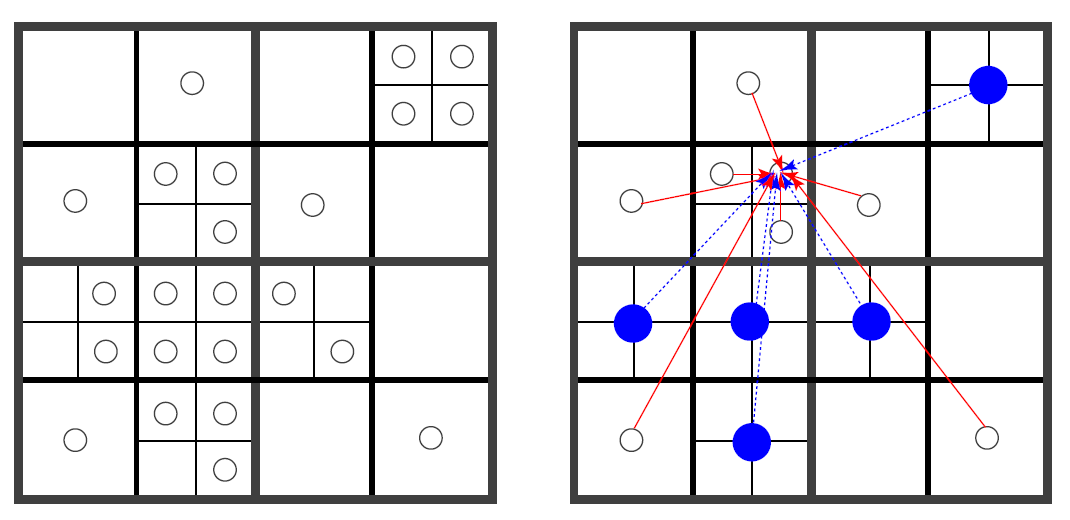
\includegraphics[width=0.8\textwidth,keepaspectratio]
  {research/makino/fig01.png}
  \caption{Basic idea of tree algorithm}
  \locallabel{fig:fig01}
\end{figure}


%% \begin{figure}[tbp]
%% \centering
%%   \includegraphics[width=0.8\textwidth,keepaspectratio]
%%   {research/makino/fig02.png}
%%   \caption{XXX}
%%   \locallabel{fig:fig02}
%% \end{figure}

%% \begin{figure}[tbp]
%% \centering
%%   \includegraphics[width=0.8\textwidth,keepaspectratio]
%%   {research/makino/fig03.png}
%%   \caption{XXX}
%%   \locallabel{fig:fig03}
%% \end{figure}

In the case of the particle-based methods, physical values are
assigned to particles, while the partial differential equation is
approximated by the interactions between particles. 

Both methods are widely used, and they have their advantages and
disadvantages. The computational cost of grid-based schemes is
generally lower than that of particle-based methods with similar
number of freedoms. Thus, if an near-uniform grid structure is
appropriate for the problem to be solved, grid-based methods perform
better. 

The advantage of the particle-based methods comes from the fact that
they use "Lagrangian" schemes, in which the particles move following
the motion of the fluid in the case of the CFD calculation. In the
case of grid-based methods, we generally use "Eulerian" schemes, in
which the grid points do not move. 

There are three points in which the Lagrangian schemes are better than
Eulerian schemes.  One is that the Lagrangian schemes are, to some
extent, adaptive to the requirement of the accuracy, since when a
low-density region is compressed to become high density, Second one is
that the timestep criteria are quite different. In the case of the
Lagrangian schemes, the timestep is determined basically by local
sound velocity, while in the Eulerian scheme by global velocity. Thus,
if a relatively cold fluid is moving very fast, the timestep for the
Eulerian schemes can be many orders of magnitude shorter than that for
Lagrangian schemes. Finally, in the case of fast-moving
low-temperature fluid, the required accuracy would be very high for
Eulerian scheme, since the error comes from the high velocity, while
that error would be transferred to internal energy of the fluid
element which is much smaller than that of the kinetic motion.

Of course, there are disadvantages of Lagrangian schemes. The primary
one is the difficulty of construction of such schemes in two or higher
dimensions.  In the case of one-dimensional calculation, it is easy to
move grid points following the motion of the fluid, but in two or
higher dimensions, the grid structure would severely deform if we let
the grid points follow the flow. Thus, we have to reconstruct the grid
structure every so often. This requirement causes the program to
become complex. Moreover, reconstruction of the grid structure (so
called remeshing) means we lose numerical accuracy.

Particle-based methods "solve" this difficulty by not requiring any
mesh. In particle-based methods, particles interact with its
neighboring particles, not through some connection through grid, but
through distance-dependent kernel functions. Thus, there is no need of
remeshing. As a result, particle-based schemes are simple to
implement, and can give reasonable results even when the deformation
is very large. Another important advantage is that it is relatively
easy to achieve high efficiency with large-scale particle-based
simulation.

In the case of grid-based schemes, in order achieve some adaptivity to
the solution, we have to use either irregular grid or regular grid
with adaptive mesh refinment. In both cases, adaptivity breaks the
regularity of the mesh structure, resulting in non-contiguous access
to the main memory. In the case of the particle-based schemes, it does
require some irregular memory access, but it is relatively
straightforward to make good use of spacial locality, and thereby
achieving high efficiency. Similarly, very high parallel performance
can be achieved.

However, it has its own problems. In the case of the SPH method, it
has been known that the standard scheme cannot handle the contact
discontinuity well. It also require rather strong artificial
viscosity, which results in very low effective Reynolds number.

Thus, in many fields of computational sciences, many groups are
working on implementation of high-performance particle-based
simulation codes for their specific problem.

One serious problem here is that, high-performance, highly-parallel
simulation codes for particle-based simulations are becoming more and
more complex, in order to make full use of modern supercomputers. We
need to distribute particles to many computing nodes in an appropriate
way, so that the communication between nodes is minimized and at the
same time near-optimal load balance is achieved. Within each nodes, we
need to write an efficient code to find neighbor particles, rearrange
data structure so that we can make good use of the locality, make good
use of multiple cores and SIMD units within each core.

Even for the case of very simple particle-particle interaction such as the Lenard-Jones potential or Coulomb potential, the calculation code tends to be very large, and since the large fraction of the code is written to achieve a high efficiency on a specific architecture, it becomes very hard to port a code which is highly optimized to one architecture to another architecture.

Our goal is to develop a "universal" software that can be applied to a variety of problems whose scales are vastly different.  
In designing such universal software, it is important to ensure that it runs efficiently on highly parallel computers such as the K computer. Achieving a good load balance with particle-based simulation is a difficult task, since using a regular spatial decomposition method causes severe load imbalance, though this works well for grid-based software. Consequently, we have developed an adaptive decomposition method that is designed to work in a way that the calculation time on each node is almost the same, resulting in near-optimal load balance.

The strategy to develop such a universal software is as follows.

We first construct an highly parallel and very efficient implementation of the TreePM algorithm for  gravitational N-body problem. This is actually not a completely new implementation, but the GreeM code developed by researchers of the Strategic Program for Innovative Research (SPIRE) Field 5 “The origin of matter and the universe. In collaboration with the Field 5 researchers, we improve the
efficiency of the code and study the issues of  the data structure, domain decomposition, load balance strategy etc.

In the second stage, we will develop a prototype of the parallel particle simulation platform. We will design the platform so that it can be used for multiple physical systems. In practice, we consider the following three applications as the initial targets.

1. Gravitational N-body simulation
2. Smoothed Particle Hydrodynamics 
3. Molecular Dynamics

In the meantime, we will also investigate the way to improve the performance and accuracy of the current particle-based algorithms for hydrodynamics.

\section{Research Results and Achievements}

As we stated in section 2, we are working on the three major subtopics, in order to develop the universal platform for particle simulations.

In the following, we briefly describe the status of our research in each subtopic.

\subsection{High-performance gravitational N-body solver.}

We use the TreePM algorithm as the basic method for the evaluation of
gravitational interaction between particles. TreePM is a combination
of the tree method and the $\rm P^3M$ (particle-particle
particle-mesh) scheme. Figure  \localref{fig:fig01} shows the basic idea of the tree
algorithm. The space is divided into a hierarchical octree structure
(quadtree in the figure). Division is stopped when a cell contains one
or no particle. When we calculate the force on a particle, we evaluate
the force from a group of particles, with size larger for more distant
particles. In this way, we can reduce the calculation cost from O(N2)
to O(N log N).


The tree algorithm is widely used, but when the periodic boundary
condition is applied, we can actually use a more efficient efficient
scheme, since we can calculate the long-range, periodic term using
FFT. The $\rm P^3M$ scheme has been used for such problem, but it has
the serious problem that when the density contrast becomes high, the
calculation cost increases very quickly. The TreePM scheme solves this
difficulty by using the tree algorithm to evaluate the forces from
nearby particles. Even when there are very large number of neighbor
particles, the calculation cost does not increase much, since the
calculation cost of the neighbor force is proportional to the
logarithm of the number of neighbors.



In order to map the problem to the distributed-memory parallel
computer such as the K computer, we adopted the approach to divide the
space into domains and assign particles in one domain to one
calculation node. We used the orthogonal recursive multisection method
developed by the team leader some years ago. It is the generalization
of the orthogonal recursive bisection (ORB), which has been widely
used in many parallel implementations of the tree algorithm.

With ORB, we recursively divide space into two halves, each with the
same number of particles. An obvious disadvantage of the ORB approach
is that it can utilize the computing nodes of integral powers of
two. Thus, in the worst case we can use only half of the available
nodes.

The difference between the multisection method and the ORB is that
with the multisection method we allow the divisions to arbitrary
number of domains, instead of bisection. This would allow too many
possible divisions. In our current implementation, we limit the number
of levels to three, and make the numbers of divisions at all levels as
close as possible. Thus, our domain decomposition is topologically a
simple three-dimension grid. This fact makes the multisection method
well suited to the machines with the 3D torus network like the K
computer.



We have developed a "reference code" for gravitational N-body
simulation on the K computer. This code is fairly well optimized for
the K computer, and shows quite good scalability for even for
relatively small-size problems. The asymptotic speed per timestep for
large number of nodes is around 7ms. This speed is comparable to that
of highly optimized molecular dynamics codes on K, even though our
code is designed to handle highly inhomogenous systems.

We used this code as the reference implementation for more generalized
particle simulation platform which will be described in the next
subsection.

\subsection{Particle Simulation Platform.}

In FY 2014, We have completed and released Version 1.0 of the particle
simulation platform, which we call FDPS (Framework for Developing
Particle Simulator). In FY 2015, we have applied a number of
improvements to FDPS. 

The basic idea of FDPS is that the application developer (or the user)
specified the way the particles interact with each other, and the rest
is taken care by FDPS. Here, "the rest" includes domain decomposition
and re-distribution of particles, evaluation of interactions between
particles, including those in different domains (different MPI
processes, for example).

In practice, there are many additional details the user should
give. Consider a relatively simple case of particles interacting with
softened 1/r potential. There are a number of small but important
points one has to decide on. For example, what algorithm should be
used for the interaction calculation? Even if we limit the
possibilities to reasonably adaptive schemes for open boundary
problems, we have the choice between Barnes-Hut tree and FMM. For both
algorithms, there are many different ways to parallelize them on
distributed-memory parallel computers. Also, there are infinitely many
variations for the time integration schemes.

The base layer of FDPS offers the domain decomposition based on the
recursive multisection algorithm, with arbitrary weighting function
for the load balancing. It also offers the parallel implementation of
interaction calculation between particles.

The domain decomposition part takes the array of particles on each
node as the main argument. It then generates an appropriate domain for
each node, redistribute particles according to their locations, and
returns.

The interaction calculation part takes the array of particles, the
domain decomposition structure, and the specification of the
interaction between particles as main arguments. The actual
implementation of this part need to take into account a number of
details. For example, the interaction can be of long-range nature,
such as gravity, Coulomb force, and interaction between computational
elements in the boundary element method (BEM). In this case, the user
should also provide the way to construct approximations such as the
multipole expansion and the way to estimate error. The interaction
might be of short-range nature, with either particle-dependent or
independent cutoff length. In these cases, the interaction calculation
part should be reasonably efficient in finding neighbor particles.

We have successfully implemented all of these functionalities in FDPS
version 1.0. (https://github.com/FDPS/FDPS). Using FDPS, a
gravitational N-body simulation code can be written in 120 lines, and
that code is actually fully scalable even to full-node runs on K
computer. For SPH calculations, we have also achieved similar scaling.

FDPS is implemented as a class template library in C++ language. It
receives the class definition of particles and a function (or multiple
functions in the case of complex interactions) to evaluate the
interaction between particles. When a user program is compiled with
the FDPS library, the class template is instantiated with the
user-specified definition of the particle class. Thus, even though the
FDPS library functions are generic ones not specialized to a
particular definition of particles, it behaves as if it is a
specialized one.

The measured performance of applications developed using FDPS is quite
good. Both for gravity-only calculation and SPH calculation,
weak-scaling performance is practically perfect, up to the full-node
configuration of K computer. Moreover, the measured efficiency, in
terms of the fraction of the peak floating-point performance, is also
very high. It is around 50\% for gravity-only calculation. For SPH
calculations, at the time of writing the performance is around 10\%.

In FY 2015, we have extended FDPS in several important directions.
The first one is the improvement of the strong scaling. The algorithm
used for the domain decomposition contains one serial bottleneck. The
``sampling'' algorithm used in FDPS 1.0 works well only when the
average number of particles per MPI process is significantly larger
than the total number of MPI processes. We developed a new parallel
algorighm, in which $O(p^{1/3}$ MPI processes are used to decompose
the computational domain. Here $p$ is the total number of MPI
processes. Thus now the requirement for the number of particle is
relaxed from larger than $p$ to  larger than $p^{2/3}$. Now we can
achieve pretty good performance for around 1 billion particles, on the
full nodes of K computer. Previously we need near 100 billion particle
to achieve good efficiency.

The second one is the addition of new interface method to interaction
calculation function, which allows  efficient use of accelerator
hardware such as GPGPU or Intel MIC. In order to achieve high
performance on accelerators, it is important to pass a large chunk of
work at one time. In order to achieve this goal, in the current
version of FDPS the CPU creates the list of multiple interaction
lists, and send all of them at once so that the overhead of the
initialization of the accelerator would not become a bottleneck.
This interface has been tested on NVIDIA GPGPUs as well as the PEZY-SC
processor.








\subsection{Improvements on SPH.}


SPH (Smoothed Particle Hydrodynamics) has been used in many field,
including astrophysics, mechanical engineering and civil
engineering. Recently, however, it was pointed out that the standard
formulation of SPH has numerical difficulty at the contact
discontinuity. The reason is that the formulation of the standard SPH
requires that the density is differentiable, which is by definition no
the case at the contact discontinuity.

We have been working on the possible solution on this problem.  One approach is to reformulate SPH so that it does not use the density in the right-hand side of the equation of motion.  We one way to achieve the density independence.  We constructed an SPH scheme which uses artificial density-like quantity as the base of the volume estimator. It evolves through usual continuity equation, but with additional diffusion term. Thus, we can guarantee the continuity and differentiability of this quantity, except at the initial condition or at the moment when two fluid elements contact with each other. This scheme seems to work extremely well, and we are currently working on the way to extend this scheme so that it can handle free surface accurately.

We are also working on a completely different approach, in which we replace the SPH formulation to evaluate the gradient to other schemes. SPH has a known problem that its kernel estimate contains O(1) error, since the summation of contributions from neighbor particles is not guaranteed to be unity. The reason why SPH uses this mathematically inconsistent formulation is to achieve symmetry and conservation. In SPH discretization, interaction between two particles is symmetric, which guarantees the conservation of linear and angular momenta. However, the use of SPH approximation resulted in rather low accuracy, which limits the reliability of the results obtained using SPH. We are experimenting with several different schemes which can achieve much higher accuracy, while losing some of the nice features of SPH such as the symmetry of interaction.

%% Text for research Results and achievements. Journal-artcile~\cite{sample-journal}.
%% Conference-paper~\cite{sample-conference}.
%% Invited-talk~\cite{sample-invited}.

%% For cross referencing, use \verb|\locallabel| and \verb|\localref| to avoid conflicting names defined by other groups. For example, a figure can be referenced as Figure~\localref{fig:sample-label1}.

%% \begin{figure}
%% \centering
%%   \includegraphics[width=0.5\textwidth,keepaspectratio,natwidth=193,natheight=40]
%%   {sample_division/sample_group/test1.png}
%%   \caption{Caption for a sample figure}
%%   \locallabel{fig:sample-label1}
%% \end{figure}

\section{Schedule and Future Plan}

We plan to improve the performance of FDPS further in FY 2015. In particular, we plan to extend the API so that the users of FDPS can easily use heterogeneous machines such as machines with GPGPUs or Intel MIC.


%%% DO NOT EDIT BELOW

\section{Publications}

%\printbibliography[keyword=journal, heading=subbibliography, title={Journal Articles}, prefixnumbers={1-}, resetnumbers=true]
%\printbibliography[keyword=proceedings, heading=subbibliography, title={Conference Papers}, prefixnumbers={2-}, resetnumbers=true]
%\printbibliography[keyword=invited, heading=subbibliography, title={Invited Talks}, prefixnumbers={3-}, resetnumbers=true]
%\printbibliography[keyword=poster, heading=subbibliography, title={Posters and Presentations}, prefixnumbers={4-}, resetnumbers=true]
%\printbibliography[keyword=deliverable, heading=subbibliography, title={Patents and Deliverables}, prefixnumbers={5-}, resetnumbers=true]

\printbibliography[keyword=journal, heading=subbibliography, title={Journal Articles}, resetnumbers=true]
\printbibliography[keyword=proceedings, heading=subbibliography, title={Conference Papers}]
\printbibliography[keyword=invited, heading=subbibliography, title={Invited Talks}]
\printbibliography[keyword=poster, heading=subbibliography, title={Posters and Presentations}]
\printbibliography[keyword=deliverable, heading=subbibliography, title={Patents and Deliverables}]

\end{refsection}
